\documentclass[11pt]{article}

\usepackage[letterpaper,margin=1in,headheight=14pt,headsep=0.3in,footskip=0.4in]{geometry}
\usepackage{amsmath,amssymb,mathtools}
\usepackage{needspace}
\usepackage{fancyhdr}
\usepackage{tikz}
\usetikzlibrary{arrows.meta,decorations.markings,patterns,calc}

% --- Layout safety: nothing runs off the margin or the page bottom ---
\emergencystretch=3em
\allowdisplaybreaks
\setlength{\parindent}{0pt}
\setlength{\parskip}{0.6em}
\raggedbottom

% --- Page numbers: top and bottom outer-right corners, with rules ---
\pagestyle{fancy}
\fancyhf{}
\fancyhead[R]{\thepage}
\fancyfoot[R]{\thepage}
\renewcommand{\headrulewidth}{0.4pt}
\renewcommand{\footrulewidth}{0.4pt}

% --- Section styling ---
\usepackage{titlesec}
\titleformat{\section}{\Large\bfseries}{}{0pt}{}[\vspace{0.15em}\titlerule]
\titleformat{\subsection}{\large\bfseries}{}{0pt}{}
\titlespacing*{\section}{0pt}{1.6em}{0.8em}
\titlespacing*{\subsection}{0pt}{1.2em}{0.4em}

% --- Notation ---
\newcommand{\ih}{\hat{\imath}}
\newcommand{\jh}{\hat{\jmath}}
\newcommand{\kh}{\hat{k}}
\newcommand{\eps}{\varepsilon_0}
\newcommand{\dd}{\,\mathrm{d}}

\begin{document}

\begin{center}
  {\LARGE\bfseries EMT Study Guide 1}
\end{center}

This study guide will mainly follow Pollack \& Stump's, with some inspiration from Griffith's and Dr.\ Ray's notes. 
It will start with a brief review of Pollack chapter 2, but really will begin with chapter 3.
Practice problems are at the end. Some are based on tophat questions, but mostly they will be in the style of the tutorials.

\section{Math Review}

\subsection{Vectors}

\begin{center}
\begin{tikzpicture}[scale=1, >=Stealth]
  % axes
  \draw[->] (0,0) -- (0,3.2) node[above] {$z$};
  \draw[->] (0,0) -- (3.9,0) node[right] {$y$};
  \draw[->] (0,0) -- (-3.1,-1.9) node[below left] {$x$};
  % point and projections
  \coordinate (P) at (1.6,1.9);
  \coordinate (Pxy) at (1.6,-1.0);
  \draw[->] (0,0) -- (P) node[above right] {$P$};
  \node[above left, xshift=2pt] at (0.8,0.95) {$\bar{x}$};
  \draw[dashed] (0,0) -- (Pxy);
  \draw[dashed] (P) -- (Pxy);
  \draw[dashed] (0,1.9) -- (P);
  \draw[dashed] (Pxy) -- (-1.63,-1.0);
  \draw[dashed] (Pxy) -- (3.2,0);
  % primed labels
  \node[left] at (0,1.9) {$z'$};
  \node[above] at (3.2,0) {$y'$};
  \node[below left] at (-1.63,-1.0) {$x'$};
  % angles
  \draw ([shift=(49.9:0.8)]0,0) arc (49.9:90:0.8);
  \node at (0.22,1.05) {$\theta$};
  \draw (211.6:0.55) arc (211.6:328:0.55);
  \node at (0,-0.85) {$\phi$};
\end{tikzpicture}
\end{center}

\[
  \bar{x} = x'\,\ih + y'\,\jh + z'\,\kh
\]
Remember right-hand rule, $\ih\times\jh=\kh$, so don't swap $x$ and $y$ axes.

\[
  \bar{A}\cdot\bar{B} = \sum_i A_i B_i
\]
because $\ih\cdot\jh=0$, $\jh\cdot\kh=0$, $\ih\cdot\kh=0$ (orthonormal basis).

\[
  \bar{A}\times\bar{B} =
  \begin{vmatrix}
    \ih & \jh & \kh\\
    A_x & A_y & A_z\\
    B_x & B_y & B_z
  \end{vmatrix}
\]

\[
  \bar{A}\cdot(\bar{B}\times\bar{C}) = (\bar{A}\times\bar{B})\cdot\bar{C}
  \qquad\qquad
  \bar{A}\times(\bar{B}\times\bar{C}) = \bar{B}(\bar{A}\cdot\bar{C}) - \bar{C}(\bar{A}\cdot\bar{B})
\]

\[
  \bar{A}\cdot\bar{B} = |\bar{A}||\bar{B}|\cos\theta
  \qquad\qquad
  \bar{A}\times\bar{B} = |\bar{A}||\bar{B}|\sin\theta\,\hat{n}
\]

\[
  \nabla f = \frac{\partial f}{\partial x}\,\ih + \frac{\partial f}{\partial y}\,\jh + \frac{\partial f}{\partial z}\,\kh
\]
$\nabla f$ is a vector. $f$ is a scalar function.

\[
  \nabla\cdot\bar{F}(\bar{x}) = \frac{\partial F_x}{\partial x} + \frac{\partial F_y}{\partial y} + \frac{\partial F_z}{\partial z}
\]
$\nabla\cdot\bar{F}$ is a scalar. $\bar{F}(\bar{x})$ is a vector function.

\[
  \nabla^2 f = \nabla\cdot(\nabla f) = \frac{\partial^2 f}{\partial x^2} + \frac{\partial^2 f}{\partial y^2} + \frac{\partial^2 f}{\partial z^2}
\]

\[
  \nabla\times\bar{F} =
  \begin{vmatrix}
    \ih & \jh & \kh\\
    \dfrac{\partial}{\partial x} & \dfrac{\partial}{\partial y} & \dfrac{\partial}{\partial z}\\[1ex]
    F_x & F_y & F_z
  \end{vmatrix}
\]

%=====================================================================
\subsection{Integral Theorems}

\textbf{Gauss's Theorem}
\[
  \oint_S \bar{F}\cdot\dd\bar{A} = \int_V \nabla\cdot\bar{F}\dd^3x
\]
Everything produced inside must come out through the boundary surface $S$. Or, total flow out of $\bar{F}$ through $S$ is the sum of ``sources'' minus ``sinks.''

\textbf{Stokes's Theorem}
\[
  \oint_C \bar{F}\cdot\dd\bar{\ell} = \int_S (\nabla\times\bar{F})\cdot\dd\bar{A}
\]

%=====================================================================
\subsection{Cylindrical Coordinates \hfill \normalfont\normalsize Pg 34}

\begin{align*}
  \nabla f &= \hat{r}\,\frac{\partial f}{\partial r} + \hat{\phi}\,\frac{1}{r}\frac{\partial f}{\partial \phi} + \kh\,\frac{\partial f}{\partial z}\\[1ex]
  \nabla\cdot\bar{F} &= \frac{1}{r}\frac{\partial}{\partial r}(rF_r) + \frac{1}{r}\frac{\partial F_\phi}{\partial \phi} + \frac{\partial F_z}{\partial z}\\[1ex]
  \nabla^2 f &= \frac{1}{r}\frac{\partial}{\partial r}\!\left(r\frac{\partial f}{\partial r}\right) + \frac{1}{r^2}\frac{\partial^2 f}{\partial \phi^2} + \frac{\partial^2 f}{\partial z^2}
\end{align*}

Curl:
\begin{align*}
  (\nabla\times\bar{F})_r &= \frac{1}{r}\frac{\partial F_z}{\partial \phi} - \frac{\partial F_\phi}{\partial z}\\[1ex]
  (\nabla\times\bar{F})_\phi &= \frac{\partial F_r}{\partial z} - \frac{\partial F_z}{\partial r}\\[1ex]
  (\nabla\times\bar{F})_z &= \frac{1}{r}\frac{\partial}{\partial r}(rF_\phi) - \frac{1}{r}\frac{\partial F_r}{\partial \phi}
\end{align*}

\[
  x = r\cos\phi \qquad\qquad y = r\sin\phi \qquad\qquad z = z
\]

%=====================================================================
\subsection{Spherical Coordinates \hfill \normalfont\normalsize Pg 36}

\begin{align*}
  \nabla f &= \hat{r}\,\frac{\partial f}{\partial r} + \hat{\theta}\,\frac{1}{r}\frac{\partial f}{\partial \theta} + \hat{\phi}\,\frac{1}{r\sin\theta}\frac{\partial f}{\partial \phi}\\[1ex]
  \nabla\cdot\bar{F} &= \frac{1}{r^2}\frac{\partial}{\partial r}(r^2F_r) + \frac{1}{r\sin\theta}\frac{\partial}{\partial \theta}(\sin\theta\,F_\theta) + \frac{1}{r\sin\theta}\frac{\partial F_\phi}{\partial \phi}
\end{align*}

More can be found on Pg 36, but I don't feel like copying it here.

%=====================================================================
\section{Chapter 3: Principles of Electrostatics}

\subsection{Coulomb's Law}

Force on $q_1$ due to $q_2$:
\[
  F_1 = \frac{1}{4\pi\eps}\,\frac{q_1q_2}{r^2}\,\hat{r}
\]
If $\vec{r} = \bar{x}_1 - \bar{x}_2$, then
\[
  F_1 = \frac{q_1q_2}{4\pi\eps}\,\frac{\bar{x}_1-\bar{x}_2}{|\bar{x}_1-\bar{x}_2|^3}
\]
$\dfrac{1}{4\pi\eps}$ has units of $\dfrac{\mathrm{N\,m^2}}{\mathrm{C}^2}$ $= 8.99\times10^{9}\,\dfrac{\mathrm{N\,m^2}}{\mathrm{C}^2}$. \quad C (coulomb) $=$ 1 amp second.

\subsection{Superposition}

\[
  F_q = \sum_{k=1}^{N}\frac{q\,q_k}{4\pi\eps}\,\frac{\bar{x}-\bar{x}_k}{|\bar{x}-\bar{x}_k|^3}
\]

\subsection{Electric Field}

Definition is force exerted on small test $q$ at $\bar{x}$:
\[
  \bar{E}(\bar{x}) = \lim_{q\to0}\frac{\bar{F}}{q}
  \qquad\qquad
  \bar{F}_q = q\,\bar{E}(\bar{x})
\]
\[
  \bar{E}(\bar{x}) = \sum_{k=1}^{N}\frac{q_k}{4\pi\eps}\,\frac{\bar{x}-\bar{x}_k}{|\bar{x}-\bar{x}_k|^3}
\]
All electrostatics can be derived from Coulomb's and superposition.

\subsection{Field of Charge Continuum}

Denote volume charge density $\rho(\bar{x}')$ at location $\bar{x}'$:
\[
  \bar{E}(\bar{x}) = \frac{1}{4\pi\eps}\int \frac{\bar{x}-\bar{x}'}{|\bar{x}-\bar{x}'|}\,\rho(\bar{x}')\dd^3x'
\]
If $\Phi$ is a scalar function,
\[
  \nabla\Phi = \left(\frac{\partial\Phi}{\partial x},\,\frac{\partial\Phi}{\partial y},\,\frac{\partial\Phi}{\partial z}\right)
\]
\[
  (\nabla\times\nabla\Phi)_x = \frac{\partial}{\partial y}\frac{\partial\Phi}{\partial z} - \frac{\partial}{\partial z}\frac{\partial\Phi}{\partial y} = 0
\]
Same for $y$ and $z$. So $\nabla\times\nabla\Phi = 0$.

Note
\[
  -\nabla\frac{1}{|\bar{x}-\bar{x}'|} = \frac{\bar{x}-\bar{x}'}{|\bar{x}-\bar{x}'|^3}
\]
so,
\[
  \bar{E}(\bar{x}) = -\nabla\frac{1}{4\pi\eps}\int\frac{\rho(\bar{x}')\dd^3x'}{|\bar{x}-\bar{x}'|} = -\nabla V(\bar{x}) \;\Rightarrow\; -\nabla^2V = \frac{\rho}{\eps}
\]
$V$ is a scalar function, so
\[
  \nabla\times\bar{E} = \nabla\times(-\nabla V) = 0
\]
because curl of gradient is always $0$. So $\nabla\times\bar{E}=0$.

%=====================================================================
\Needspace{8\baselineskip}
\subsection{Electric Potential and Boundary Conditions}

\[
  \nabla\cdot\bar{E} = \frac{\rho}{\eps}
  \qquad\text{and}\qquad
  -\nabla^2V = \frac{\rho}{\eps}
\]
\[
  \bar{E}(\bar{x}) = -\nabla\frac{1}{4\pi\eps}\int\frac{\rho(\bar{x}')\dd^3x'}{|\bar{x}-\bar{x}'|}
\]
where
\[
  V(\bar{x}) = \frac{1}{4\pi\eps}\int\frac{\rho(\bar{x}')}{|\bar{x}-\bar{x}'|}\dd^3x'
\]
is the electric potential. For point charges it is
\[
  V(\bar{x}) = \frac{1}{4\pi\eps}\sum_{k=1}^{N}\frac{q_k}{|\bar{x}-\bar{x}'|}
\]

$\nabla\times\bar{E}=0$, so the tangential component of $\bar{E}$ must be continuous across a surface $S$. $\bar{E}_n$, normal to the surface, is continuous unless there is a surface charge; then there is a discontinuity of $\sigma/\eps$.

Use Gauss's law to prove that:

\begin{center}
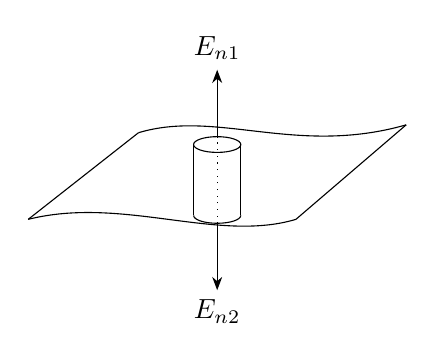
\begin{tikzpicture}[>=Stealth]
  % sheet
  \draw (-3,-0.4) .. controls (-1.8,-0.1) and (-0.6,-0.7) .. (0.4,-0.4);
  \draw (-1.6,0.7) .. controls (-0.6,1.0) and (0.4,0.4) .. (1.8,0.8);
  \draw (-3,-0.4) -- (-1.6,0.7);
  \draw (0.4,-0.4) -- (1.8,0.8);
  % pillbox
  \draw (-0.6,0.55) ellipse (0.3 and 0.1);
  \draw (-0.9,0.55) -- (-0.9,-0.35);
  \draw (-0.3,0.55) -- (-0.3,-0.35);
  \draw (-0.9,-0.35) arc (180:360:0.3 and 0.1);
  % normals
  \draw[->] (-0.6,0.65) -- (-0.6,1.5) node[above] {$E_{n1}$};
  \draw[->] (-0.6,-0.45) -- (-0.6,-1.3) node[below] {$E_{n2}$};
  \draw[dotted] (-0.6,-0.45) -- (-0.6,0.65);
\end{tikzpicture}
\end{center}

\begin{align*}
  \oint\bar{E}\cdot\dd\bar{A} &= \frac{Q_{\mathrm{enc}}}{\eps}
\end{align*}
\begin{align*}
  \oint\bar{E}\cdot\dd\bar{A} &= \frac{\sigma\dd A}{\eps}\\[1ex]
  E_{n1}\dd A - E_{n2}\dd A &= \frac{\sigma\dd A}{\eps}\\[1ex]
  E_{n1} - E_{n2} &= \frac{\sigma}{\eps}
\end{align*}

For an infinite plane,
\[
  \bar{E}(\bar{x}) =
  \begin{cases}
    \dfrac{\sigma}{2\eps}\,\kh & z>0\ \ \text{(above)}\\[2ex]
    -\dfrac{\sigma}{2\eps} & z<0\ \ \text{(below)}
  \end{cases}
\]
Discontinuity of $\sigma/\eps$.

%=====================================================================
\subsection{Dirac Delta Function}

For every continuous $f(x)$, define $\delta(x)$ such that
\[
  \int_{-\infty}^{\infty}\delta(x)f(x)\dd x = f(0)
\]
To satisfy this, $\delta(x)$ must $=0$ $\forall\,x\neq0$ and
\[
  \int_{-\infty}^{\infty}\delta(x)\dd x = 1
\]
This seems insane, and it kinda is, but watch this:

Let
\[
  d_\tau(t) =
  \begin{cases}
    \dfrac{1}{2\tau} & -\tau<t<\tau\\[1.5ex]
    0 & \text{otherwise}
  \end{cases}
\]

\begin{center}
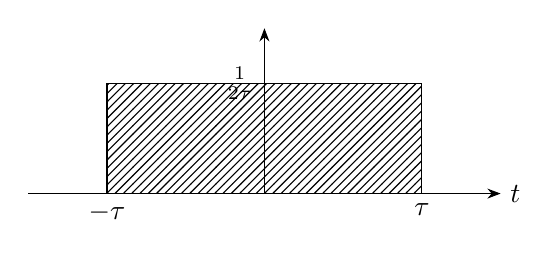
\begin{tikzpicture}[>=Stealth]
  \fill[pattern=north east lines] (-2,0) rectangle (2,1.4);
  \draw (-2,0) -- (-2,1.4) -- (2,1.4) -- (2,0);
  \draw[->] (-3,0) -- (3,0) node[right] {$t$};
  \draw[->] (0,0) -- (0,2.1);
  \node[left] at (0,1.4) {$\tfrac{1}{2\tau}$};
  \node[below] at (-2,0) {$-\tau$};
  \node[below] at (2,0) {$\tau$};
\end{tikzpicture}
\end{center}

\[
  \int_{-\infty}^{\infty}d_\tau(t)\dd t = 1
\]
Now imagine what happens when $\tau\to0$. $\displaystyle\int_{-\infty}^{\infty}d_\tau(t)\dd t=1$ still holds.
\[
  \delta(t) = \lim_{\tau\to0}d_\tau(t)
\]
Mathematically, this notation is horrendous and you shouldn't use it around mathematicians. Instead you would use the limit notation
\footnote{No actual function can be $0$ everywhere except one point and still have integral $1$, since changing a function at a single point doesn't change its integral. Mathematicians instead treat $\delta$ as shorthand for what happens in the limit, after integrating against a smooth function $f$:
$\lim_{\tau\to0}\int_{-\infty}^{\infty}d_\tau(t)f(t)\dd t=f(0)$.
This is the only property of $\delta$ you ever actually use.}, 
Anyway!
\[
  \delta(x) =
  \begin{cases}
    \infty & x=0\\
    0 & x\neq0
  \end{cases}
  \qquad\text{and}\qquad
  \int_{-\infty}^{\infty}\delta(x)\dd x = 1
\]
More generally,
\[
  \int_{-\infty}^{\infty}\delta(x-c)f(x)\dd x = f(c)
\]
Examples:
\[
  \int_{-\infty}^{\infty}x^2\,\delta(2-x)\dd x = (2)^2 = 4
\]
\[
  \int_0^{\infty}x^2\,\delta(x+2)\dd x
\]
$c=-2$, but $-2$ isn't in $[0,\infty]$, so this is $0$.

\[
  \delta^3(\bar{x}) = \delta(x)\,\delta(y)\,\delta(z)
\]
has units $\mathrm{m}^{-3}$. Generally, units of $\dfrac{1}{\text{input unit}}$.

%=====================================================================
\Needspace{10\baselineskip}
\subsection{Green's Function}

Green's function of $-\nabla^2$ is $G(\bar{x}-\bar{x}')$:
\[
  -\nabla^2G(\bar{x}-\bar{x}') = \delta^3(\bar{x}-\bar{x}')
\]
along with boundary condition $G\to0$ at infinity.
\[
  G(\bar{x}-\bar{x}') = \frac{1}{4\pi|\bar{x}-\bar{x}'|}
  \qquad\qquad \text{proof on Pg 64}
\]
Pollack writes (3.58):
\[
  \nabla\cdot\bar{E} = \frac{1}{\eps}\int\left[-\nabla^2G(\bar{x}-\bar{x}')\right]\rho(\bar{x}')\dd^3x'
\]

\subsection{Electric Potential}

$V(\bar{x})$ is a scalar function such that
\[
  \bar{E}(\bar{x}) = -\nabla V(\bar{x})
\]
$V(\bar{x})$ has units of volts, $1\,\mathrm{V} = 1\,\mathrm{J/C}$ (work/unit charge).
\[
  V(\bar{x}) = \frac{1}{4\pi\eps}\int\frac{\rho(\bar{x}')\dd^3x'}{|\bar{x}-\bar{x}'|}
\]
For a point charge at the origin,
\[
  V(\bar{x}) = \frac{q}{4\pi\eps\,r}
\]
Another way to construct $V(\bar{x})$ is
\[
  V(\bar{x}) = -\int_\Gamma\bar{E}\cdot\dd\bar{\ell}
\]
$V(\bar{x})$ is the work that must be done by an external force acting against electric force to move unit charge from $\bar{x}_0$ to $\bar{x}$ along $\Gamma$ (path).

Note:
\[
  -\int_{\infty}^{a}\bar{E}\cdot\dd\bar{\ell} = \int_{a}^{\infty}\bar{E}\cdot\dd\bar{\ell}
\]
$V(\bar{x})$ doesn't depend on the path $\Gamma$ taken.

%=====================================================================
\subsection{Energy of Electric Field}

Note about Poisson's
\[
  -\nabla^2V = \frac{\rho}{\eps}:
\]
This, with boundary conditions, determines $V(\bar{x})$.

Suppose you have a stationary configuration of point charges and you move a charge $Q$ from $a$ to $b$. How much work will it take? At any point the force due to $\bar{E}$ is $Q\bar{E}$, so you must exert $-Q\bar{E}$.
\begin{align*}
  W = \int_a^b\bar{F}\cdot\dd\bar{\ell} &= -Q\int_a^b\bar{E}\cdot\dd\bar{\ell}\\
  &= Q\left[V(b)-V(a)\right]
\end{align*}
If you bring in $Q$ from far far away to $\bar{r}$,
\[
  W = Q\left[V(\bar{r})-V(\infty)\right]
\]
So if you set the reference point at $\infty$, $W=QV(\bar{r})$ (the work you must do).

Some notes on $V(\bar{r})$:
\[
  V(\bar{r}) = -\int_{\bar{x}_0}^{\bar{r}}\bar{E}\cdot\dd\bar{\ell}
\]
where $\bar{x}_0$ is our reference point where $V(\bar{x}_0)=0$, so $V(\bar{r})$ depends on what we set as our reference point $\bar{x}_0$. In this sense it is like altitude. Sea level? Height above terrain? $V$ is all about \underline{difference}.

The potential energy (not the same as electric potential) with respect to the reference point is defined as $-W$, so
\[
  U_q(\bar{x}) = q\,V(\bar{x})
\]
Potential energy is well defined for any force $F$ as long as $\nabla\times F=0$.

Total electrostatic energy of set of charges:
\[
  U = \frac{1}{2}\sum_{i\neq j}\frac{q_iq_j}{4\pi\eps\,|\bar{x}_i-\bar{x}_j|}
\]

%=====================================================================
For a charge distribution,
\[
  U = \frac{1}{2}\int\frac{\rho(\bar{x})\rho(\bar{x}')}{4\pi\eps\,|\bar{x}-\bar{x}'|}\dd^3x\dd^3x'
\]
or
\[
  U = \frac{1}{2}\int\rho(\bar{x})V(\bar{x})\dd^3x
\]
Pollack and Stump write
\[
  \rho V = -\eps(\nabla^2V)V = -\eps\,\nabla\cdot(V\nabla V) + \eps(\nabla V)^2
\]
I don't have a good derivation for this, but they use this to justify total energy:
\[
  U = \frac{\eps}{2}\int E^2\dd^3x
\]
and energy density of $\bar{E}$ is
\[
  u_E(\bar{x}) = \frac{\eps}{2}E^2(\bar{x})
\]

\subsection{Multipole Expansion}

Point charge at origin:
\[
  V(\bar{x}) = \frac{q}{4\pi\eps\,r}
  \qquad\qquad
  \bar{E}(\bar{x}) = \frac{q\,\hat{r}}{4\pi\eps\,r^2}
\]
For two charges,
\[
  V(\bar{x}) = \frac{q_1}{4\pi\eps\,|\bar{x}-\bar{x}_1|} + \frac{q_2}{4\pi\eps\,|\bar{x}-\bar{x}_2|}
\]
For $r\gg r_1$ \& $r\gg r_2$,
\[
  V(\bar{x}) = \frac{1}{4\pi\eps}\left\{\frac{Q}{r} + \frac{\hat{r}\cdot\bar{P}}{r^2} + \frac{\hat{r}\cdot Q_2\cdot\hat{r}}{r^3}\right\}
\]
(Deriving this is a good exercise.)

$Q$ total charge, \quad $\bar{P} = q_1\bar{x}_1 + q_2\bar{x}_2$,
\[
  Q_2 = \frac{q_1}{2}\left[3\bar{x}_1\bar{x}_1 - r_1^2 I\right] + \frac{q_2}{2}\left[3\bar{x}_2\bar{x}_2 - r_2^2 I\right]
\]

\Needspace{16\baselineskip}
\textbf{Example 12 from P\&S:}

\begin{center}
\begin{tikzpicture}[>=Stealth]
  \draw[->] (0,0) -- (0,3.6);
  \draw[->] (0,0) -- (4.2,0);
  \fill (0,0.9) circle (1.5pt) node[right] {$q_1$};
  \fill (0,1.8) circle (1.5pt) node[right] {$q_2$};
  \node[left] at (0,0.9) {$d_1$};
  \node[left] at (0,1.8) {$d_2$};
  \fill (3.2,3.2) circle (1.5pt) node[right] {$P$};
  \draw[dashed] (0,0) -- (3.2,3.2);
  \node[above left] at (1.6,1.6) {$r$};
  \draw (0,0.7) arc (90:45:0.7);
  \node at (0.28,0.95) {};
  \node at (0.38,0.32) {$\theta$};
\end{tikzpicture}
\end{center}

\[
  V(r,\theta) = \frac{1}{4\pi\eps}\left\{\frac{q_1}{\sqrt{r^2-2rd_1\cos\theta+d_1^2}} + \frac{q_2}{\sqrt{r^2-2rd_2\cos\theta+d_2^2}}\right\}
\]
\[
  \hat{r}\cdot\bar{P} = (q_1d_1+q_2d_2)\cos\theta
\]
\[
  Q_2 = \frac{q_1d_1^2+q_2d_2^2}{2r^3}\,(3\cos\theta-1) \qquad \text{(for example 12)}
\]

%=====================================================================
\subsection{Dipoles}

Dipole vectors go from negative charge to positive. $\bar{P}=q\bar{d}$. When $d\to0$ this is a point-like dipole. If you take the origin as the dipole position, all other terms in the multipole expansion other than dipole are $0$.
\[
  V(\bar{x}) = \frac{\bar{P}\cdot\hat{r}}{4\pi\eps\,r^2}
\]

\begin{center}
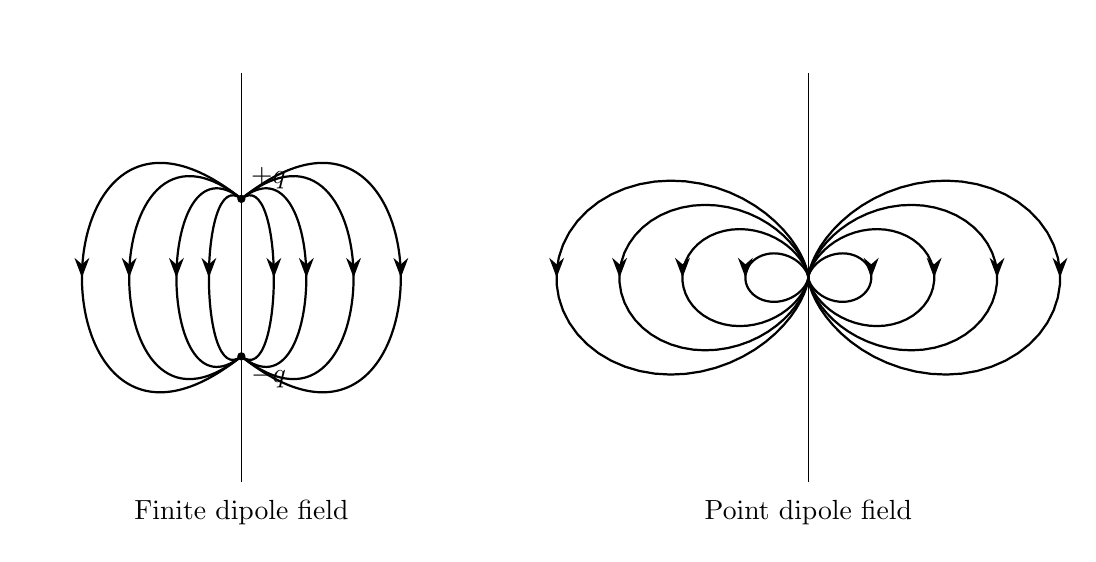
\begin{tikzpicture}[>=Stealth,
  fl/.style={thick, postaction={decorate},
    decoration={markings, mark=at position 0.5 with {\arrow{Stealth[length=2.5mm]}}}}]
  % ---- finite dipole ----
  \begin{scope}[xshift=-3.6cm]
    \draw (0,-2.6) -- (0,2.6);
    \fill (0,1) circle (1.5pt) node[above right] {$+q$};
    \fill (0,-1) circle (1.5pt) node[below right] {$-q$};
    \foreach \w in {0.55,1.1,1.9,2.7} {
      \draw[fl] (0,1) .. controls (\w,{1+0.8*\w}) and (\w,{-1-0.8*\w}) .. (0,-1);
      \draw[fl] (0,1) .. controls (-\w,{1+0.8*\w}) and (-\w,{-1-0.8*\w}) .. (0,-1);
    }
    \node[below] at (0,-2.7) {Finite dipole field};
  \end{scope}
  % ---- point dipole ----
  \begin{scope}[xshift=3.6cm]
    \draw (0,-2.6) -- (0,2.6);
    \foreach \a in {0.8,1.6,2.4,3.2} {
      \draw[fl, domain=0:180, samples=60, variable=\t]
        plot ({\a*sin(\t)^3},{\a*sin(\t)^2*cos(\t)});
      \draw[fl, domain=0:180, samples=60, variable=\t]
        plot ({-\a*sin(\t)^3},{\a*sin(\t)^2*cos(\t)});
    }
    \node[below] at (0,-2.7) {Point dipole field};
  \end{scope}
\end{tikzpicture}
\end{center}

Not really sure why, but P\&S talk about some molecules and
\[
  1\ \text{Debye} = 3.33\times10^{-30}\ \mathrm{C\,m}
\]
\[
  \bar{E}(\bar{x}) = -\nabla V = \frac{3\hat{r}(\bar{P}\cdot\hat{r})-\bar{P}}{4\pi\eps\,r^3}
\]
For $\bar{P}$ at origin, $\bar{P}=P_0\kh$, $\bar{E}$ in spherical is
\[
  \bar{E}(\bar{x}) = -\nabla V = \frac{P_0}{4\pi\eps\,r^3}\left(2\cos\theta\,\hat{r}+\sin\theta\,\hat{\theta}\right)
\]

\subsection{Moments of General Charge Distribution}

\[
  Q = \sum_{k=1}^{N}q_k
  \qquad\quad
  \bar{P} = \sum_{k=1}^{N}q_k\bar{x}_k
  \qquad\quad
  Q_2 = \sum_{k=1}^{N}\frac{q_k}{2}\left(3\bar{x}_k\bar{x}_k - r_k^2I\right)
\]
For situations with $\rho(\bar{x}')$:
\begin{gather*}
  Q = \int\rho(\bar{x}')\dd^3x'
  \qquad\quad
  \bar{P} = \int\bar{x}'\rho(\bar{x}')\dd^3x'\\[1ex]
  Q_2 = \int\frac{1}{2}\left(3\bar{x}'\bar{x}' - r^2I\right)\rho(\bar{x}')\dd^3x'
\end{gather*}
If charge is $0$, $\bar{P}$ is independent of origin. If origin is moved to $\bar{x}_0$, then
\[
  \bar{P}_0 = \int(\bar{x}'-\bar{x}_0)\rho(\bar{x}')\dd^3x' = \bar{P}-Q\bar{x}_0
\]

%=====================================================================
\subsection{Torque on a Dipole}

A dipole in a field $\bar{E}$ experiences a torque that twists the dipole to align with $\bar{E}$. The torque is
\[
  \bar{N} = \int\bar{x}\times\dd\bar{F} = \int\bar{x}\times\bar{E}(\bar{x})\rho(\bar{x})\dd^3x
\]
If $\bar{E}$ is constant on the scale of $\rho$ (point-like dipole),
\[
  \bar{N} = \bar{P}\times\bar{E}
\]

%=====================================================================
\section{Chapter 4: Electrostatic Properties of Conductors}

\begin{itemize}
  \item $\bar{E}$ field is $0$ inside a conductor at equilibrium.
  \item Potential is constant inside conductor at equilibrium.
  \item Charge density is zero inside conductor at equilibrium.
  \item We can specify net charge or potential for a conductor.
  \item At the surface, $E_{\text{tangent}}=0$ and $E_{\text{normal}}=\sigma/\eps$.
  \newpage
  \item Potential is uniquely determined up to a constant when
  \begin{enumerate}
    \item[a)] the charge densities and
    \item[b)] either potentials or total charge of conductors
  \end{enumerate}
  are specified.
\end{itemize}

\[
  V(\bar{x})=V_0 \qquad \text{Dirichlet boundary condition.}
\]
If surface charge density is known,
\[
  -\hat{n}\cdot\nabla V = \frac{\sigma}{\eps} \qquad \text{Neumann.}
\]

$\bar{E}$ is $0$ in any conductor cavity regardless of $\bar{E}$ outside.
\Needspace{14\baselineskip}
\begin{center}
\begin{tikzpicture}[>=Stealth]
  \def\gausscyl#1#2#3#4#5{%
    \draw (#1-#4,#2) -- (#1-#4,#3);
    \draw (#1+#4,#2) -- (#1+#4,#3);
    \draw (#1,#3) ellipse (#4 and #5);
    \draw (#1-#4,#2) arc (180:360:#4 and #5);
    \draw[dashed] (#1-#4,#2) arc (180:0:#4 and #5);}
  \draw[->] (0,-1.3) -- (0,3.3) node[above] {$z$};
  % top plate
  \draw (-1.9,1.7) rectangle (2.4,2.2);
  \node[above] at (0.9,2.2) {$Q_{2u}$};
  \node[below] at (0.9,1.7) {$Q_{2l}$};
  \node[right] at (2.4,1.95) {$V_0$};
  \draw[dashed] (3.1,1.7) -- (4.0,1.7) node[right] {$z=d$};
  \draw (-2.1,1.7) -- (-2.2,1.7) -- (-2.2,2.2) -- (-2.1,2.2);
  \node[left] at (-2.2,1.95) {$d_2$};
  % bottom plate
  \draw (-1.9,-0.5) rectangle (2.4,0);
  \node[above] at (0.9,0) {$Q_{1u}$};
  \node[below] at (0.9,-0.5) {$Q_{1l}$};
  \draw[dashed] (2.4,0) -- (4.0,0) node[right] {$z=0$};
  \node[below right] at (2.4,0) {$V=0$};
  \draw (-2.1,-0.5) -- (-2.2,-0.5) -- (-2.2,0) -- (-2.1,0);
  \node[left] at (-2.2,-0.25) {$d_1$};
  % ground
  \draw (2.0,-0.5) -- (2.0,-1.0);
  \draw (1.7,-1.0) -- (2.3,-1.0);
  \draw (1.8,-1.1) -- (2.2,-1.1);
  \draw (1.9,-1.2) -- (2.1,-1.2);
  % Gauss cylinder
  \gausscyl{-1.2}{-0.25}{1.95}{0.3}{0.1}
\end{tikzpicture}
\end{center}

\[
  V(z) = V_0\,\frac{z}{d} \qquad \text{in region between plates}
\]
\[
  E = -\nabla V = -\frac{V_0}{d}
\]

Cylindrical Gauss surface:

\Needspace{14\baselineskip}
Cylindrical Gauss surface:

\begin{center}
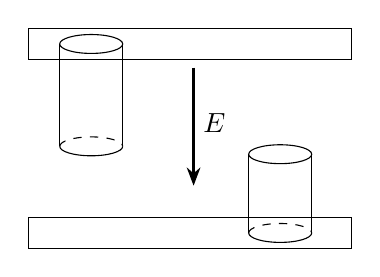
\begin{tikzpicture}[>=Stealth]
  \def\gausscyl#1#2#3#4#5{%
    \draw (#1-#4,#2) -- (#1-#4,#3);
    \draw (#1+#4,#2) -- (#1+#4,#3);
    \draw (#1,#3) ellipse (#4 and #5);
    \draw (#1-#4,#2) arc (180:360:#4 and #5);
    \draw[dashed] (#1-#4,#2) arc (180:0:#4 and #5);}
  % top plate
  \draw (-2.2,2.0) rectangle (1.9,2.4);
  \gausscyl{-1.4}{0.9}{2.2}{0.4}{0.12}
  % field
  \draw[->, thick] (-0.1,1.9) -- (-0.1,0.4);
  \node[right] at (-0.1,1.2) {$E$};
  % bottom plate
  \draw (-2.2,-0.4) rectangle (1.9,0.0);
  \gausscyl{1.0}{-0.2}{0.8}{0.4}{0.12}
\end{tikzpicture}
\end{center}

Top:
\begin{align*}
  \pi r^2E &= \frac{Q_{\mathrm{enc}}}{\varepsilon_0}\\[1ex]
  -\pi r^2\varepsilon_0\,\frac{V_0}{d} &= Q_{\mathrm{enc}}\\[1ex]
  \sigma_{2l} &= -\varepsilon_0\,\frac{V_0}{d}
\end{align*}

Bottom:
\[
  \bar{E}\cdot\mathrm{d}\bar{A} < 0 \quad\text{because they oppose each other}
\]
\begin{align*}
  -\pi r^2E &= \frac{Q_{\mathrm{enc}}}{\varepsilon_0}\\[1ex]
  \pi r^2\varepsilon_0\,\frac{V_0}{d} &= Q_{\mathrm{enc}} \;\Rightarrow\; \sigma_{1u} = \varepsilon_0\,\frac{V_0}{d}
\end{align*}

Two plates holding equal \& opposite charges $\pm Q$ form a capacitor. Capacitance depends on geometry only.
\begin{align*}
  C &= \frac{Q}{V}\\[1ex]
    &= \frac{A\,\dfrac{\varepsilon_0V_0}{d}}{V_0\,\dfrac{z}{d}} = \frac{\varepsilon_0A}{z}
\end{align*}
But here $z=d$:
\[
  \frac{\varepsilon_0A}{d} = C
\]

\subsection{Energy of Capacitors}

\begin{center}
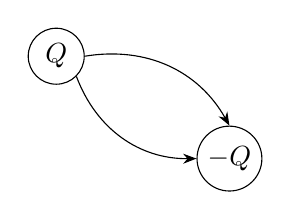
\begin{tikzpicture}[>=Stealth]
  \node[draw, circle, inner sep=3pt] (a) at (0,0) {$Q$};
  \node[draw, circle, inner sep=2pt] (b) at (2.2,-1.3) {$-Q$};
  \draw[->] (a.east) to[bend left=35] (b.north);
  \draw[->] (a.south east) to[bend right=35] (b.west);
\end{tikzpicture}
\end{center}

\[
  U = \frac{1}{2}\int\rho V\,\mathrm{d}^3x
\]
Because charge lies on surface,
\[
  U = \frac{1}{2}\int\sigma V\,\mathrm{d}A
\]
\[
  U_1 = -QV_1/2 \qquad\qquad U_2 = QV_2/2
\]
\[
  U_{\mathrm{total}} = QV/2 \qquad\qquad V = V_2 - V_1
\]
\[
  U = \frac{1}{2}QV=\frac{1}{2}CV^2=\frac{Q^2}{2C}
\]
% requires: amsmath, tikz

\textbf{Method of Images:}

\hspace{1.5em}A charge external of a conductor creates an $E$ field which enduces a charge on the surface of the conductor. The resulting net $E$ field outside the conductor can be modeled with a ficticious equal and opposite charge at an equal distance to the boundary.

\begin{minipage}{\linewidth}
\centering
\begin{tikzpicture}
  \draw[thick] (-3,0) -- (3,0);
  \foreach \x in {-2.8,-2.5,...,2.9} \draw (\x,0) -- ++(-0.2,-0.2);
  \draw[dashed, thick, dash pattern=on 1.5pt off 4pt] (0,1.6) -- (0,-1.6);
  \fill (0,1.6) circle (1.5pt);
  \node[left=3pt] at (0,1.6) {$z_0$};
  \node[right=3pt] at (0,1.6) {$q$};
  \fill (0,-1.6) circle (1.5pt);
  \node[left=3pt] at (0,-1.6) {$-z_0$};
  \node[right=3pt] at (0,-1.6) {$-q$};
\end{tikzpicture}
\end{minipage}

You can easily write $V(x,y,z)$ and then $\vec{E} = -\nabla V$. using $\bar{E}(r) = \dfrac{\sigma}{\epsilon_0}\cdot\hat{n}$ where $r = \sqrt{x^2+y^2}$ you can show
\[
  \sigma(r) = \dfrac{-q\,z_0}{2\pi\left(r^2+z_0^2\right)^{3/2}}
\]

$*$ Try showing total charge on plane is $-q$

with a dipole:

\begin{minipage}{\linewidth}
\centering
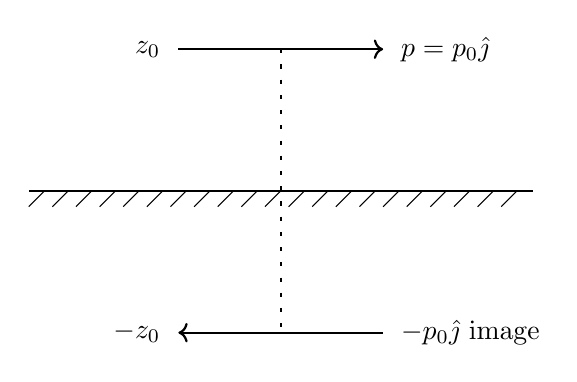
\begin{tikzpicture}
  \draw[thick] (-3.2,0) -- (3.2,0);
  \foreach \x in {-3.0,-2.7,...,3.1} \draw (\x,0) -- ++(-0.2,-0.2);
  \draw[dashed, thick, dash pattern=on 1.5pt off 4pt] (0,1.8) -- (0,-1.8);
  \draw[->, thick] (-1.3,1.8) -- (1.3,1.8);
  \node[left=3pt] at (-1.3,1.8) {$z_0$};
  \node[right=3pt] at (1.3,1.8) {$p = p_0\hat{\jmath}$};
  \draw[->, thick] (1.3,-1.8) -- (-1.3,-1.8);
  \node[left=3pt] at (-1.3,-1.8) {$-z_0$};
  \node[right=3pt] at (1.3,-1.8) {$-p_0\hat{\jmath}$\ image};
\end{tikzpicture}
\end{minipage}

\[
  \bar{E}(0,0,z) = \dfrac{p_0\hat{\imath}}{4\pi\epsilon_0}
  \left[\dfrac{-1}{(z-z_0)^3} + \dfrac{1}{(z-z_0)^3}\right]
\]

\begin{minipage}{\linewidth}
\centering
multiple image charges\par\medskip
\begin{tikzpicture}
  \draw[thick] (0,2.4) -- (0,0) -- (3,0);
  \foreach \y in {0.2,0.5,...,2.3} \draw (0,\y) -- ++(-0.2,-0.2);
  \foreach \x in {0.2,0.5,...,2.9} \draw (\x,0) -- ++(-0.2,-0.2);
  \fill (1.4,1.2) circle (1.5pt);   \node[right=3pt] at (1.4,1.2) {$q$};
  \fill (1.4,-1.2) circle (1.5pt);  \node[right=3pt] at (1.4,-1.2) {$-q$};
  \fill (-1.4,1.2) circle (1.5pt);  \node[left=3pt] at (-1.4,1.2) {$-q$};
  \fill (-1.4,-1.2) circle (1.5pt); \node[left=3pt] at (-1.4,-1.2) {$+q$};
\end{tikzpicture}
\end{minipage}

\textbf{Spherical Charges}

We can find $V$ outside of a charged sphere using Laplace's equation $\nabla^2 V = 0$. We have boundary conditions $V(a) = V_0$, $V(\infty) = 0$. (Sphere has radius $a$.)

Laplace's equation becomes
\[
\frac{1}{r^2}\frac{d}{dr}\left(r^2\frac{dV}{dr}\right) = 0
\]

We can try $V(r) \propto r^p$ with $p = 0$ or $p = -1$. Why?

Try $V = r^p$:
\begin{align*}
\frac{dV}{dr} &= p\,r^{p-1} \\
r^2\frac{dV}{dr} &= p\,r^{p-1}\,r^2 = p\,r^{p+1} \\
r^2\frac{d^2V}{dr^2} &= p(p+1)\,r^p \\
\frac{d^2V}{dr^2} &= \frac{1}{r^2}\,p(p+1)\,r^p = 0
\end{align*}

So $p$ must be either $0$ or $-1$.

If $p = 0$ then $V$ is constant. If $p = -1$ then $V \propto 1/r$, but we can add a constant to $V$ without violating $\nabla^2 V = 0$.

So
\[
V = B + \frac{A}{r}
\]

$V(\infty) = 0 \Rightarrow B = 0$. $V(a) = V_0$ requires $A = V_0\,a$.

So
\[
V(r) = V_0\,\frac{a}{r} \quad \text{for } r \geq a
\]


\newpage
\section{Practice Problems}

% --- Problem format (define once, here, before the first problem) ---
\newcounter{problem}
\newcommand{\problem}[1][]{%
  \Needspace{6\baselineskip}%
  \refstepcounter{problem}%
  \subsection{Problem \theproblem\ifx&#1&\else\ (#1)\fi}%
}
% \problem[Topic]
% Problem statement here.
%
% \problem[Topic]
% Problem statement here.
\end{document}